\IfFileExists{solve_stats/language_stats.pdf}{%
  \begin{frame}[c]{Language stats}
    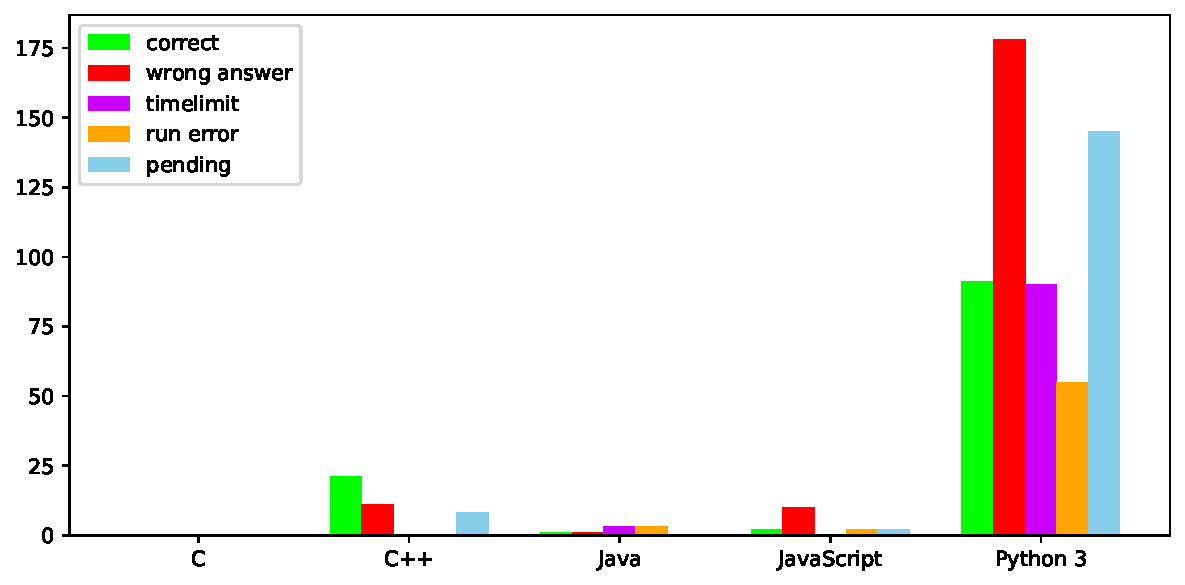
\includegraphics[width=\textwidth]{solve_stats/language_stats}%
  \end{frame}
}

\begin{frame}{Random facts}
    \begin{block}{Jury work}
      \begin{itemize}[<+->]
        \item 12 problèmes (KARWa 2024 : 13 problèmes)
        % git rev-list --all -- main | wc -l
        \item 157 commits (KARWa 2024 : 193)
        % bt stats
        \item 611 test cases secrets (KARWa 2024 : 693) ($\approx 51$ par problème !)
        \item 39 solutions du jury (KARWa 2024 : 28)
        % cd main ; for dir in */ ; do echo "$dir $(cloc --by-file ${dir}submissions/accepted | tail -n 4 | head -n 1)" ; done
        % cd main; for dir in */ ; do cloc --by-file ${dir}submissions/accepted | tail -n 4 | head -n 1 | tr -s ' ' | cut -d ' ' -f 4 ; done
        \item Le nombre minimum de lignes dont le jury a eu besoin pour résoudre tous les problèmes est
        \[ 29+6+3+23+15+6+1+33+3+17+12+13 = 161. \]
        En moyenne $13$ lignes par problème.
      \end{itemize}
    \end{block}
    %\footnotetext{\emph{After} codegolfing}
\end{frame}
